\documentclass[11pt,a4paper]{article}

\usepackage[utf8]{inputenc}
\usepackage[T1]{fontenc}
\usepackage[english]{babel}
\usepackage{lmodern}

\usepackage{geometry}
\geometry{
    top=2.5cm,
    bottom=2.5cm,
    left=2.5cm,
    right=2.5cm
}

\usepackage{amsmath,amssymb}
\usepackage{booktabs}
\usepackage{array}
\usepackage{graphicx}
\usepackage{listings}
\usepackage{xcolor}
\usepackage{fancyhdr}
\usepackage{hyperref}

\pagestyle{fancy}
\fancyhf{}
\rhead{\textit{Practical 5: Regression Models}}
\lhead{\textit{Data Science --- ETSINF (UPV)}}
\cfoot{\thepage}

\lstset{
    language=R,
    basicstyle=\ttfamily\footnotesize,
    keywordstyle=\color{blue}\bfseries,
    commentstyle=\color{gray}\itshape,
    stringstyle=\color{teal},
    numbers=none,
    frame=lines,
    breaklines=true,
    breakatwhitespace=true,
    showstringspaces=false,
    captionpos=b,
    tabsize=2
}

\title{\textbf{Practical 5: Regression Models}\\[0.4ex] \Large Data Science (CDA) --- Academic Lab Report}
\author{\textbf{Enrique Sopeña} \\ 
Máster Universitari en Enginyeria Informàtica (MUIInf) \\
Escola Tècnica Superior d'Enginyeria Informàtica (ETSINF) \\ 
Universitat Politècnica de València}
\date{October 24, 2026}


\setlength{\headheight}{14pt}
\lstdefinestyle{console}{
    language={},
    literate={‘}{{\textquoteleft}}1 {’}{{\textquoteright}}1,
    basicstyle=\ttfamily\scriptsize,
    frame=single,
    keywordstyle=\color{black},
    commentstyle=\color{black},
    stringstyle=\color{black},
    columns=fullflexible,
    keepspaces=true
}
\begin{document}
\maketitle
\begin{abstract}
This report studies house-price regression using 799 observations from the supplied Zillow dataset. After removing the street column and exploring five numerical housing features, the data are split into 599 training and 200 test cases. A linear model, a regression tree, and a neural network are fitted and evaluated using root mean square error (RMSE) and mean absolute error (MAE). Cross-validation guides tree pruning and a subsequent search over neural-network size and weight decay. The original tree achieves the lowest test RMSE (141,917.68), while the tuned network has the lowest test MAE (104,403.87), only 10.45 below the tree. The tuned network substantially improves on the initial network, illustrating the benefit of controlling model complexity in this experiment.
\end{abstract}
\vspace{0.8em}\hrule\vspace{1em}

\section{Introduction and Experimental Setup}
The task is to predict the numerical price of a house from its characteristics. The supplied data contain address fields, an identifier, construction year, counts of bathrooms, bedrooms and rooms, floor area, and price. The analysis is implemented in \texttt{pract5.R}; its recorded results are stored in \texttt{salida.log} and the two comparison CSV files in \texttt{outputs/}.

The predictive models use \texttt{year}, \texttt{bath}, \texttt{bed}, \texttt{rooms}, and \texttt{SqFt}. The identifier \texttt{zpid} is excluded, and \texttt{zipcode} is treated as a geographic code rather than a quantitative measurement. The categorical location fields \texttt{city} and \texttt{state} are also excluded to retain the numerical-feature scope of the experiment. Consequently, the models do not account explicitly for geographic differences in house prices.

The following sections present implementation excerpts and recorded numerical output. Additional figures for tree complexity and the pruned tree were generated during report preparation by reproducing the same training split and tree fit; the selected complexity parameter and split counts were checked against the supplied log.

\section{Exercise 1: Loading and Inspecting the Data}
\subsection{Objective and Implementation}
The semicolon-separated file is loaded with its header, and the street information is removed as requested. The original data remain in \texttt{raw\_database}, while \texttt{database} is used for subsequent analysis. Removing the street field follows the exercise, although the remaining identifier and geographic fields mean that this operation alone is not complete de-identification.
\begin{lstlisting}
raw_database <- read.csv(
  "dataset/HousePricesData-Address-City-Features_fromZillow.csv",
  header = TRUE,
  sep = ";",
  check.names = TRUE
)

database <- subset(raw_database, select = -street)

str(database)
summary(database)
\end{lstlisting}

\subsection{Results and Discussion}
\par\noindent\begin{minipage}{\linewidth}
\begin{lstlisting}[style=console]
799 observations; 10 columns after removing street.
                Min.   Median       Mean      Max.
year            1820     1951       1951      2014
bath               1        2      2.039         7
bed                0        3      3.218        14
rooms              2        6      6.708        21
SqFt             440     1536       1792      5938
price          40074   179886     252797   1608791
\end{lstlisting}
\end{minipage}\par
The compact summary above transcribes the recorded descriptive statistics. Mean price exceeds median price, indicating a right-skewed distribution with some expensive properties. The range includes zero bedrooms and construction years up to 2014; these values are retained rather than altered without supporting metadata. The inspected file contains no missing values. No observations are removed as outliers.

\section{Exercise 2: Exploring Price Relationships}
\subsection{Objective and Implementation}
The \texttt{lattice} package is used to reshape the five predictors into a common plotting column. \texttt{make.groups()} adds the grouping variable \texttt{which}, identifying the predictor represented by each row. Temporary attachment follows the exercise procedure and is reversed immediately after constructing the plotting data.
\begin{lstlisting}
library(lattice)

attach(database)
forplot <- make.groups(
  bath = data.frame(value = bath, zipcode, city, state, price),
  year = data.frame(value = year, zipcode, city, state, price),
  bed = data.frame(value = bed, zipcode, city, state, price),
  rooms = data.frame(value = rooms, zipcode, city, state, price),
  SqFt = data.frame(value = SqFt, zipcode, city, state, price)
)
detach(database)

price_plot <- xyplot(
  price ~ value | which,
  data = forplot,
  scales = list(relation = "free"),
  xlab = "Predictor value",
  ylab = "House price",
  main = "House price versus numerical features"
)
price_plot

dir.create("outputs", showWarnings = FALSE)
pdf("outputs/price_relationships.pdf")
print(price_plot)
invisible(dev.off())
\end{lstlisting}

\subsection{Results and Discussion}
Figure~\ref{fig:prices} shows price against each predictor. Floor area and bathroom count display an overall tendency towards higher prices for larger values, with substantial variation at similar predictor values. Bedroom and room counts form vertical bands because their values are discrete. Construction year does not exhibit a simple monotonically increasing relationship: both older and newer properties include expensive cases.

These plots suggest potentially useful associations, not a definitive ranking of predictive importance or causal effects. The large spread at similar feature values is consistent with important unmodelled differences between properties. Independent panel scales accommodate the different predictor ranges.\begin{figure}[htbp]
\centering
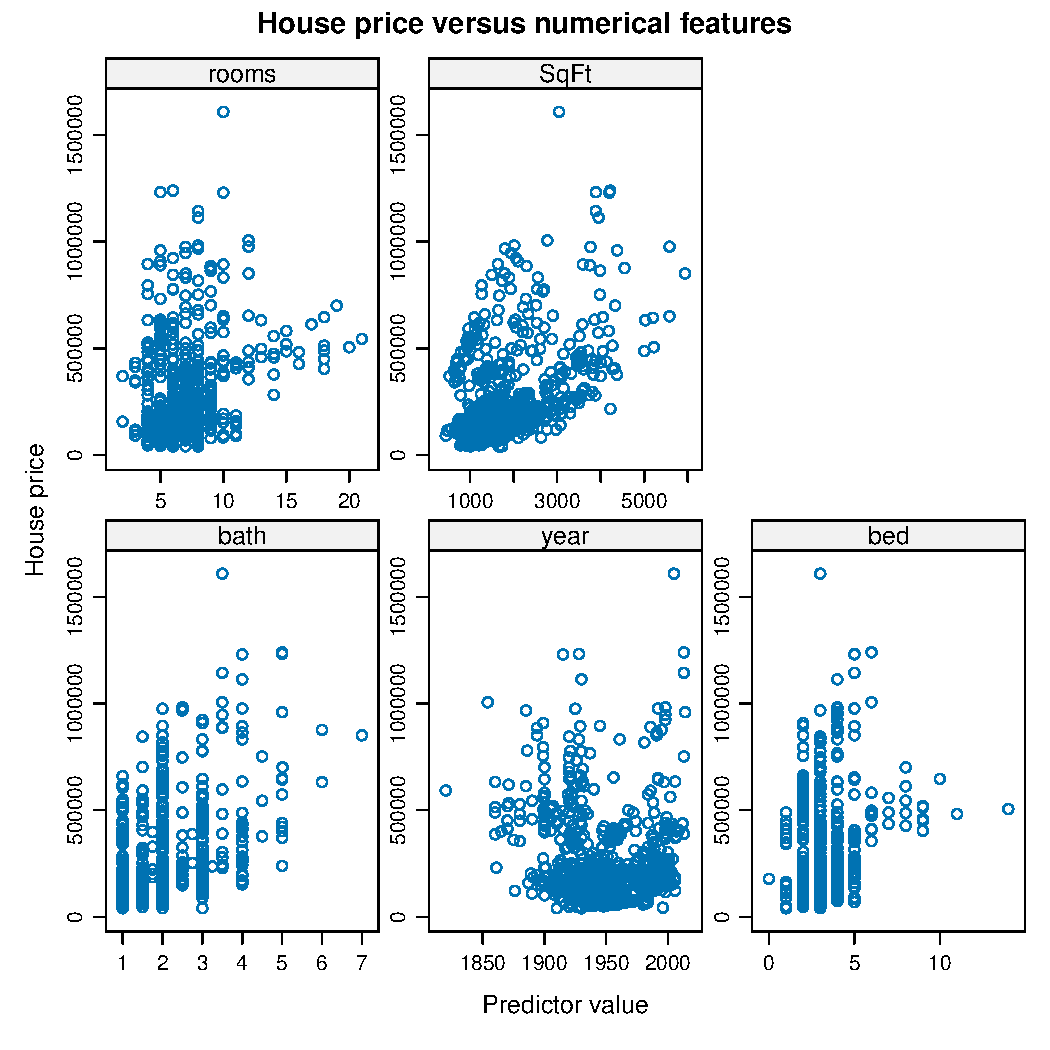
\includegraphics[page=1,width=.88\textwidth]{../outputs/price_relationships.pdf}
\caption{House price against the five numerical predictors.}
\label{fig:prices}
\end{figure}


\section{Exercise 3: Random Train/Test Split}
\subsection{Objective and Implementation}
Sampling without replacement selects approximately 75\% of the rows for training. The remaining rows form the test set, so the two subsets do not overlap. Seed 123 makes the split reproducible.
\begin{lstlisting}
set.seed(123)

train_indices <- sample(
  seq_len(nrow(database)),
  size = floor(0.75 * nrow(database)),
  replace = FALSE
)

data_train <- database[train_indices, ]
data_test <- database[-train_indices, ]

split_summary <- data.frame(
  Set = c("Training", "Test"),
  Observations = c(nrow(data_train), nrow(data_test)),
  Percentage = round(
    100 * c(nrow(data_train), nrow(data_test)) / nrow(database),
    2
  )
)

cat("\n--- Train/test split ---\n")
print(split_summary, row.names = FALSE)
\end{lstlisting}

\subsection{Results and Discussion}
\par\noindent\begin{minipage}{\linewidth}
\begin{lstlisting}[style=console]
Set Observations Percentage
 Training          599      74.97
     Test          200      25.03
\end{lstlisting}
\end{minipage}\par
The floor of $0.75\times799=599.25$ gives 599 training observations and 200 test observations. Their realised proportions are 74.97\% and 25.03\%. All models are compared on this same partition. Test prices are retained as evaluation targets and are not used for fitting or selecting the tuning configuration.

\section{Exercise 4: Fitting the Regression Models}
\subsection{Objective and Implementation}
The linear model is estimated by ordinary least squares. The CART model uses \texttt{method = "anova"} to fit a numerical response through recursive partitioning. The neural network uses 12 hidden units, direct input-to-output connections (\texttt{skip = TRUE}), and an unrestricted linear output (\texttt{linout = TRUE}). Its hidden units still allow nonlinear relationships.

Both the predictors and the target are standardised for the network, using training means and sample standard deviations only:
\[
z_j=(x_j-\mu_j)/s_j,\qquad z_y=(y-\mu_y)/s_y.
\]
The linear model and tree use the original scales. The network's fitted outputs are later transformed back with $\hat y=\mu_y+s_y\hat z_y$. The initial network uses the default zero weight decay. Seeds are reset before the tree fit and network fit to reproduce internal cross-validation and random initial weights, respectively.
\begin{lstlisting}
library(rpart)
library(nnet)

model_formula <- price ~ year + bath + bed + rooms + SqFt

model_lm <- lm(
  model_formula,
  data = data_train
)

set.seed(123)

model_tree <- rpart(
  model_formula,
  data = data_train,
  method = "anova"
)

predictors <- c("year", "bath", "bed", "rooms", "SqFt")

predictor_means <- sapply(data_train[predictors], mean)
predictor_sds <- sapply(data_train[predictors], sd)

price_mean <- mean(data_train$price)
price_sd <- sd(data_train$price)

train_scaled <- data_train[c(predictors, "price")]

train_scaled[predictors] <- scale(
  data_train[predictors],
  center = predictor_means,
  scale = predictor_sds
)

train_scaled$price <- (
  data_train$price - price_mean
) / price_sd

set.seed(123)

model_nn <- nnet(
  model_formula,
  data = train_scaled,
  size = 12,
  skip = TRUE,
  linout = TRUE,
  maxit = 1000,
  trace = FALSE
)

cat("\n--- Model training ---\n")
cat("Linear model and regression tree fitted.\n")
cat("Neural network convergence code:", model_nn$convergence, "\n")
\end{lstlisting}

\subsection{Results and Discussion}
\par\noindent\begin{minipage}{\linewidth}
\begin{lstlisting}[style=console]
Linear model and regression tree fitted.
Neural network convergence code: 0
\end{lstlisting}
\end{minipage}\par
The network reports convergence code 0, indicating that the optimiser met its stopping criterion. Convergence is not evidence of good generalisation. The three models use the same five predictors and the same 599 training cases; scaling changes their numerical representation, not the observations included.

\section{Exercise 5: Inspecting and Visualising the Models}
\subsection{Objective and Implementation}
The summaries expose different kinds of information: coefficients for the linear model, splitting rules for the tree, and connection weights for the network.
\begin{lstlisting}
print(summary(model_lm))
print(summary(model_tree))
print(summary(model_nn))

plot(model_tree, uniform = TRUE, margin = 0.1,
     main = "Regression tree for house prices")
text(model_tree, use.n = TRUE, all = FALSE, cex = 0.8)
\end{lstlisting}

\subsection{Results and Discussion}
\par\noindent\begin{minipage}{\linewidth}
\begin{lstlisting}[style=console]
Call:
lm(formula = model_formula, data = data_train)

Residuals:
    Min      1Q  Median      3Q     Max 
-429051  -99085  -36291   38946 1200656 

Coefficients:
             Estimate Std. Error t value Pr(>|t|)    
(Intercept) 4316668.3   470898.4   9.167  < 2e-16 ***
year          -2210.1      242.1  -9.130  < 2e-16 ***
bath          73111.7    12565.0   5.819 9.71e-09 ***
bed          -39204.2     8877.3  -4.416 1.19e-05 ***
rooms          7131.5     4895.8   1.457    0.146    
SqFt            103.0       15.3   6.731 3.99e-11 ***
---
Signif. codes:  0 ‘***’ 0.001 ‘**’ 0.01 ‘*’ 0.05 ‘.’ 0.1 ‘ ’ 1

Residual standard error: 172600 on 593 degrees of freedom
Multiple R-squared:  0.3566,	Adjusted R-squared:  0.3512 
F-statistic: 65.74 on 5 and 593 DF,  p-value: < 2.2e-16
\end{lstlisting}
\end{minipage}\par
The linear model has training $R^2=0.3566$ and adjusted $R^2=0.3512$. Its coefficients describe conditional associations, holding the other predictors fixed. For example, the estimated \texttt{SqFt} coefficient is approximately 103 price units per additional square foot. Negative coefficients for construction year and bedrooms should not be interpreted as causal effects; correlations between predictors and omitted location information can affect these estimates. The coefficient for \texttt{rooms} has a reported $p$-value of 0.146, which is not strong evidence of an additional linear contribution under this fitted model's assumptions.

The original tree has 14 splits and 15 leaves. Its root separates houses at \texttt{SqFt = 3030}. The first split gives training mean prices of approximately 229,962 below the threshold and 528,609 above it. These are internal-node means; predictions follow the remaining splits to a terminal leaf. The primary splitting variables are \texttt{SqFt}, \texttt{year}, \texttt{rooms}, and \texttt{bath}. A variable may receive importance through surrogate splits even if it is not used in a primary split.

The network summary identifies a 5--12--1 architecture with 90 weights. It is the least directly interpretable model: its weights do not yield a short set of conditions or a single coefficient interpretation comparable to the tree and linear model.\begin{figure}[htbp]
\centering
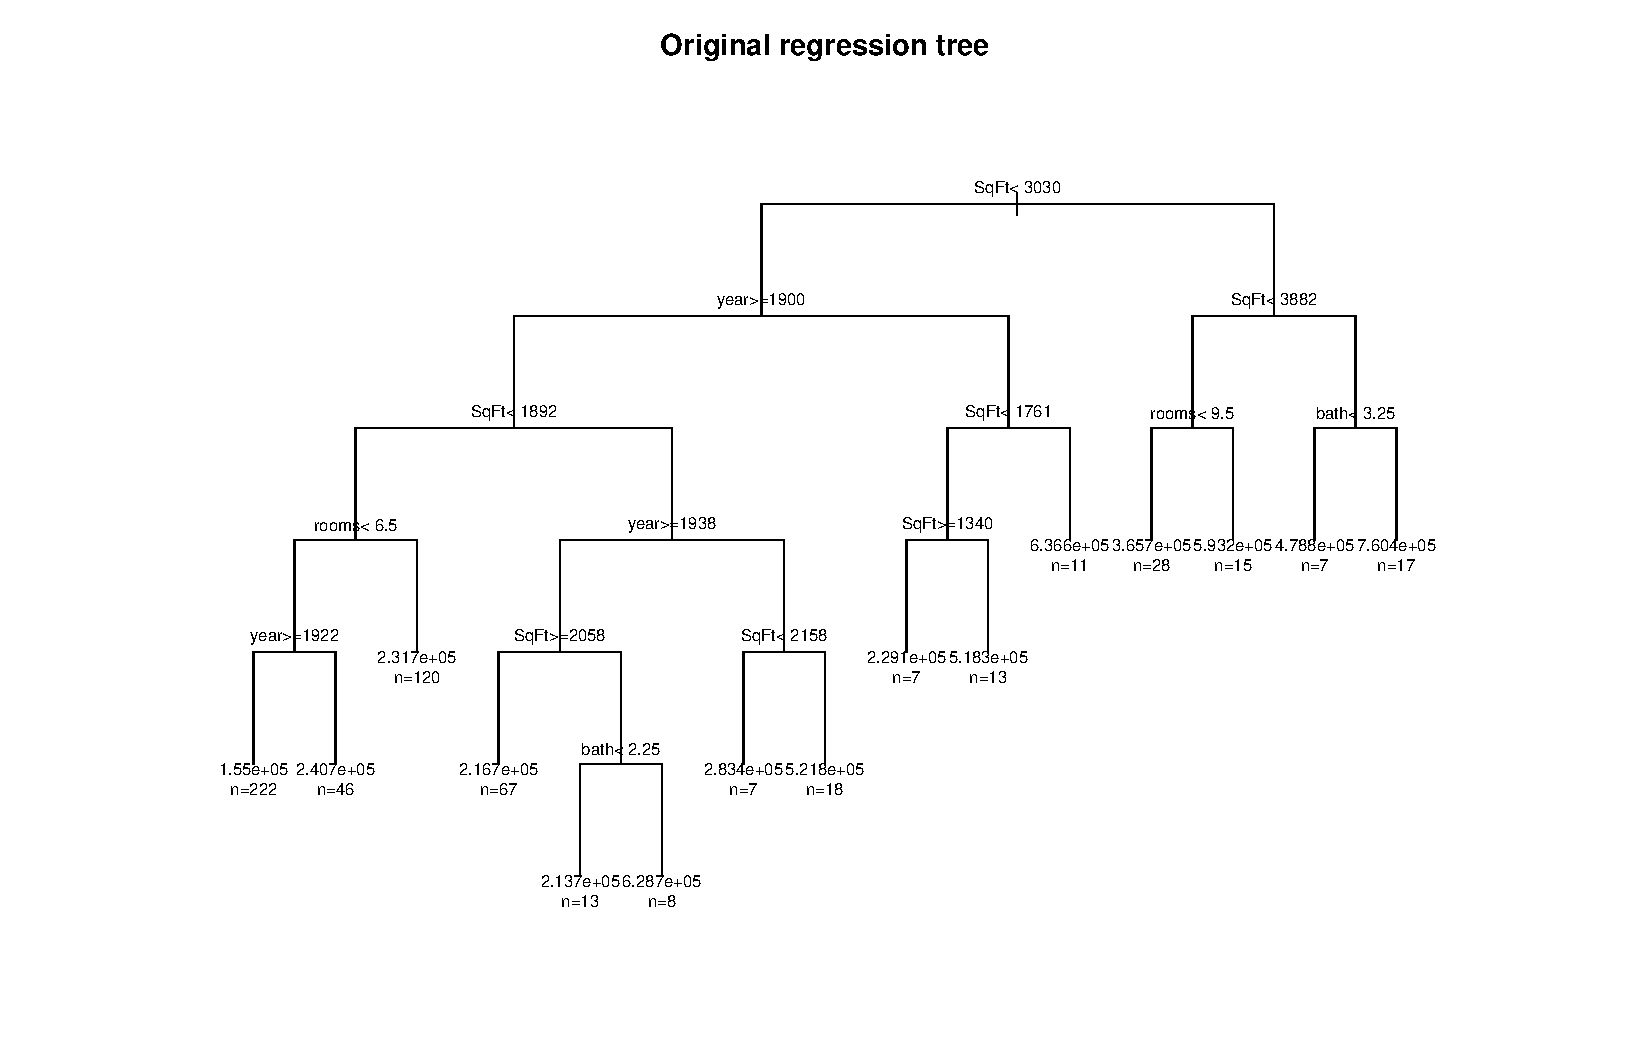
\includegraphics[page=1,width=1\textwidth]{../outputs/model_figures.pdf}
\caption{Original regression tree. Terminal nodes show predicted prices and training counts.}
\label{fig:tree}
\end{figure}


\section{Exercise 6: Pruning the Regression Tree}
\subsection{Objective and Implementation}
The complexity table is used to select a smaller tree with the one-standard-error rule. Let $i^*$ index the minimum cross-validation relative error. Eligible trees satisfy
\[
\mathrm{xerror}_i\leq\mathrm{xerror}_{i^*}+\mathrm{xstd}_{i^*}.
\]
Among them, the tree with the fewest splits is selected. This is a practical complexity-control rule, not a guarantee of equal performance.
\begin{lstlisting}
cat("\n--- Tree complexity table ---\n")
printcp(model_tree)

cp_table <- model_tree$cptable

best_row <- which.min(cp_table[, "xerror"])

error_limit <- cp_table[best_row, "xerror"] +
  cp_table[best_row, "xstd"]

# Choose the simplest tree within one standard error of the minimum.
eligible_rows <- which(cp_table[, "xerror"] <= error_limit)

selected_row <- eligible_rows[
  which.min(cp_table[eligible_rows, "nsplit"])
]

selected_cp <- cp_table[selected_row, "CP"]

model_pruned <- prune(model_tree, cp = selected_cp)

cat("\n--- Selected pruning configuration ---\n")
print(cp_table[selected_row, , drop = FALSE])

cat("\n--- Pruned tree ---\n")
print(model_pruned)
\end{lstlisting}

\subsection{Results and Discussion}
\par\noindent\begin{minipage}{\linewidth}
\begin{lstlisting}[style=console]
CP nsplit rel error    xerror       xstd
4 0.03049844      3 0.6845662 0.8134139 0.09401243

--- Pruned tree ---
n= 599 

node), split, n, deviance, yval
      * denotes terminal node

1) root 599 2.747149e+13 263366.3  
  2) SqFt< 3030 532 1.670429e+13 229961.7  
    4) year>=1899.5 501 1.228935e+13 213565.4  
      8) SqFt< 1891.5 388 6.460777e+12 188898.7 *
      9) SqFt>=1891.5 113 4.781897e+12 298261.5 *
    5) year< 1899.5 31 2.103522e+12 494947.2 *
  3) SqFt>=3030 67 5.459858e+12 528609.0 *
\end{lstlisting}
\end{minipage}\par
The minimum relative cross-validation error is 0.7333778, with standard error 0.09502515, giving a threshold of approximately 0.828403. The three-split tree has error 0.8134139 and qualifies; the two-split tree has error 0.8506876 and does not. Thus, \texttt{cp = 0.03049844} is selected, reducing the original tree from 15 to four leaves.

The four terminal predictions are approximately 188,899, 298,262, 494,947, and 528,609. They are reached using only floor area and construction year. Neither the selection rule nor the pruning operation uses test outcomes. The relative cross-validation errors are normalised squared-error quantities, not misclassification rates or monetary RMSE values.\begin{figure}[htbp]
\centering
\includegraphics[page=2,width=.85\textwidth]{../outputs/model_figures.pdf}
\caption{Tree complexity and cross-validation error.}
\label{fig:cp}
\end{figure}
\begin{figure}[htbp]
\centering
\includegraphics[page=3,width=.95\textwidth]{../outputs/model_figures.pdf}
\caption{Pruned regression tree with three splits and four leaves.}
\label{fig:pruned}
\end{figure}


\clearpage
\section{Exercise 7: Evaluating Training and Test Predictions}
\subsection{Objective and Implementation}
RMSE and MAE are calculated on the original price scale for every model:
\[
\mathrm{RMSE}=\sqrt{\frac1n\sum_{i=1}^{n}(y_i-\hat y_i)^2},
\qquad
\mathrm{MAE}=\frac1n\sum_{i=1}^{n}|y_i-\hat y_i|.
\]
RMSE gives greater influence to large errors, whereas MAE measures the average absolute deviation. Smaller values are preferable. Network test predictors are transformed with training statistics and its predictions are converted back to prices before computing either metric.
\begin{lstlisting}
# Apply the training transformation to the test predictors.
test_scaled <- as.data.frame(
  scale(
    data_test[predictors],
    center = predictor_means,
    scale = predictor_sds
  )
)

predictions_train <- list(
  Linear = predict(model_lm, newdata = data_train),
  Tree = predict(model_tree, newdata = data_train),
  Pruned_tree = predict(model_pruned, newdata = data_train),
  Neural_network = as.numeric(
    predict(model_nn, newdata = train_scaled)
  ) * price_sd + price_mean
)

predictions_test <- list(
  Linear = predict(model_lm, newdata = data_test),
  Tree = predict(model_tree, newdata = data_test),
  Pruned_tree = predict(model_pruned, newdata = data_test),
  Neural_network = as.numeric(
    predict(model_nn, newdata = test_scaled)
  ) * price_sd + price_mean
)

calculate_metrics <- function(actual, predicted) {
  errors <- actual - predicted

  c(
    RMSE = sqrt(mean(errors^2)),
    MAE = mean(abs(errors))
  )
}

train_metrics <- t(
  sapply(
    predictions_train,
    function(predicted) {
      calculate_metrics(data_train$price, predicted)
    }
  )
)

test_metrics <- t(
  sapply(
    predictions_test,
    function(predicted) {
      calculate_metrics(data_test$price, predicted)
    }
  )
)

performance <- data.frame(
  Model = names(predictions_train),
  Train_RMSE = train_metrics[, "RMSE"],
  Train_MAE = train_metrics[, "MAE"],
  Test_RMSE = test_metrics[, "RMSE"],
  Test_MAE = test_metrics[, "MAE"],
  row.names = NULL
)

cat("\n--- Model performance ---\n")
print(performance, digits = 7, row.names = FALSE)
\end{lstlisting}

\subsection{Results and Discussion}
\par\noindent\begin{minipage}{\linewidth}
\begin{lstlisting}[style=console]
Model Train_RMSE Train_MAE Test_RMSE Test_MAE
         Linear   171775.1 117006.11  144709.3 106809.8
           Tree   149769.0  99614.18  141917.7 104414.3
    Pruned_tree   177188.5 120903.45  152604.9 110848.5
 Neural_network   124487.2  86048.77  192470.3 136183.4
\end{lstlisting}
\end{minipage}\par
The initial network achieves the lowest training RMSE and MAE, but the highest test errors. This pattern is consistent with overfitting. The original tree has the lowest test RMSE (141,917.7) and MAE (104,414.3) among these four models, followed by the linear model. Pruning simplifies interpretation but increases both test errors in this split.

The linear model and both trees have lower test errors than training errors. This is possible because the two sets contain different properties and different error distributions; it is not by itself evidence of an implementation problem. The comparison describes this fixed split and does not establish statistical superiority across other samples.

\section{Exercise 8: Improving the Neural Network}
\subsection{Objective and Implementation}
The poor test performance of the initial network motivates a limited exploratory search over hidden-layer size and weight decay. Sizes 3, 6, and 12 are combined with decay values 0.01, 0.1, and 1. Weight decay penalises large weights. Five balanced folds are constructed within the training set, and the same folds are used for all nine configurations.

The search involves 45 fits, with one initialisation per configuration and fold. It uses seed 456 for fold allocation and seed $1000+\mathrm{fold}$ before fitting each network. All tuning fits allow 2,000 iterations. Test outcomes are not used to rank configurations, although the search was motivated after inspecting the baseline test results; the final test comparison should therefore be interpreted as part of an exploratory workflow rather than a fresh independent confirmation.
\begin{lstlisting}
parameter_grid <- expand.grid(
  size = c(3, 6, 12),
  decay = c(0.01, 0.1, 1)
)

set.seed(456)

fold_id <- sample(
  rep(1:5, length.out = nrow(data_train))
)
\end{lstlisting}
For each configuration, four folds form \texttt{fold\_train} and the remaining fold forms \texttt{fold\_valid}. The following excerpt is executed inside that loop. Scaling is estimated separately from each fold's training portion, preventing the validation observations from influencing preprocessing.
\begin{lstlisting}
# Fit preprocessing within each fold to avoid validation leakage.
    fold_means <- sapply(fold_train[predictors], mean)
    fold_sds <- sapply(fold_train[predictors], sd)

    fold_price_mean <- mean(fold_train$price)
    fold_price_sd <- sd(fold_train$price)

    fold_train_scaled <- as.data.frame(
      scale(
        fold_train[predictors],
        center = fold_means,
        scale = fold_sds
      )
    )

    fold_train_scaled$price <- (
      fold_train$price - fold_price_mean
    ) / fold_price_sd

    fold_valid_scaled <- as.data.frame(
      scale(
        fold_valid[predictors],
        center = fold_means,
        scale = fold_sds
      )
    )

    set.seed(1000 + fold)

    fold_model <- nnet(
      model_formula,
      data = fold_train_scaled,
      size = parameter_grid$size[i],
      decay = parameter_grid$decay[i],
      skip = TRUE,
      linout = TRUE,
      maxit = 2000,
      trace = FALSE
    )

    cv_predictions[fold_id == fold] <- as.numeric(
      predict(fold_model, newdata = fold_valid_scaled)
    ) * fold_price_sd + fold_price_mean
\end{lstlisting}
Predictions from the five validation folds are collected in their original row positions. RMSE is computed across all 599 out-of-fold residuals, rather than averaging the five fold RMSEs. MAE is reported as a secondary measure. The configuration with the lowest pooled validation RMSE is selected among those converging in all folds, with smaller networks preferred in an exact tie.
\begin{lstlisting}
eligible <- which(tuning_results$Nonconverged_fits == 0)

if (length(eligible) == 0) {
  stop("No configuration converged in every fold. Review optimisation.")
}

best_index <- eligible[
  order(
    tuning_results$CV_RMSE[eligible],
    tuning_results$size[eligible]
  )[1]
]

best_parameters <- tuning_results[best_index, ]
\end{lstlisting}
The selected configuration is refitted on all training observations using the original training scaling:
\begin{lstlisting}
set.seed(123)

model_nn_tuned <- nnet(
  model_formula,
  data = train_scaled,
  size = best_parameters$size,
  decay = best_parameters$decay,
  skip = TRUE,
  linout = TRUE,
  maxit = 2000,
  trace = FALSE
)
\end{lstlisting}

\subsection{Results and Discussion}
\par\noindent\begin{minipage}{\linewidth}
\begin{lstlisting}[style=console]
size decay  CV_RMSE   CV_MAE Nonconverged_fits
    3  0.01 179616.3 118797.8                 0
    6  0.01 185170.1 121106.4                 0
   12  0.01 229822.7 146376.4                 0
    3  0.10 176999.5 112899.4                 0
    6  0.10 190584.2 121198.7                 0
   12  0.10 193973.3 122651.5                 0
    3  1.00 172717.0 113400.4                 0
    6  1.00 173995.9 113719.0                 0
   12  1.00 173041.6 111699.8                 0

--- Selected neural network configuration ---
 size decay CV_RMSE   CV_MAE Nonconverged_fits
    3     1  172717 113400.4                 0

Tuned network convergence code: 0
\end{lstlisting}
\end{minipage}\par
All 45 validation fits and the final fit converge. The selected model has three hidden units and decay 1, with cross-validation RMSE 172,717.0 and MAE 113,400.4. The 12-unit model with decay 1 has a lower validation MAE, but it is not selected because RMSE was the specified criterion. The two configurations are close in validation RMSE, and only one initialisation per fold was tested; this search does not establish a universally optimal architecture.
\par\noindent\begin{minipage}{\linewidth}
\begin{lstlisting}[style=console]
Model Train_RMSE Train_MAE Test_RMSE Test_MAE
               Linear   171775.1 117006.11  144709.3 106809.8
                 Tree   149769.0  99614.18  141917.7 104414.3
          Pruned_tree   177188.5 120903.45  152604.9 110848.5
       Neural_network   124487.2  86048.77  192470.3 136183.4
 Tuned_neural_network   157507.3 104584.71  143576.7 104403.9
\end{lstlisting}
\end{minipage}\par
Relative to the initial network, the tuned network reduces test RMSE from 192,470.30 to 143,576.72 (25.40\%) and test MAE from 136,183.36 to 104,403.87 (23.34\%). Its training error is higher, while its test error is lower, which is consistent with reduced overfitting through the combined change in size and regularisation. The experiment does not isolate the effect of each change independently.

The original tree remains best by test RMSE. The tuned network achieves the lowest test MAE, but its advantage over the tree is only 10.45 price units, approximately 0.01\%. This negligible margin should not be presented as convincing evidence of general superiority. The CSV exports preserve the tuning and final comparison results in \texttt{outputs/neural\_network\_tuning.csv} and \texttt{outputs/model\_comparison.csv}.

\section{Conclusions}
The original regression tree provides the best test RMSE among the evaluated models and an explicit set of decision rules. Pruning makes those rules substantially shorter but does not improve test accuracy on this partition. The initial neural network fits the training data most closely and generalises poorly; a smaller regularised network substantially reduces its test errors and reaches performance close to the original tree.

The conclusions are limited to the supplied numerical predictors, one train/test partition, and the tested configurations. Geographic predictors were excluded, and the network search used one random initialisation per fold. The observed ranking should therefore be reported as an experimental result rather than a general claim that one regression method is always better.

\clearpage
\appendix
\section*{Appendix: Complete Sequential Execution Log}
\addcontentsline{toc}{section}{Appendix: Complete Sequential Execution Log}
The supplied \texttt{salida.log} is reproduced below. Its numerical output is preserved, including detailed node summaries and network weights. Report-preparation figures do not alter these recorded results.
\begin{lstlisting}[style=console]
'data.frame':	799 obs. of  10 variables:
 $ zpid   : int  956068 924224 906733 964007 74504350 81982160 7780105 7792424 7833403 56437339 ...
 $ zipcode: int  35212 35204 35215 35205 99801 85037 85021 85021 85018 2140 ...
 $ city   : chr  "Birmingham" "Birmingham" "Birmingham" "Birmingham" ...
 $ state  : chr  "AL" "AL" "AL" "AL" ...
 $ year   : int  1930 1930 1982 1919 1966 2006 1984 1974 1980 1894 ...
 $ bath   : num  2 1 2 2.5 1 3 5 2 2 3.5 ...
 $ bed    : int  3 2 3 4 1 3 5 2 2 4 ...
 $ rooms  : int  7 6 11 7 3 5 9 4 4 9 ...
 $ SqFt   : int  1732 1115 1355 2876 476 1652 3945 1625 1794 2294 ...
 $ price  : int  40745 205906 98672 325474 114726 122241 573258 239086 304824 885883 ...
      zpid              zipcode          city              state          
 Min.   :9.060e+05   Min.   : 2121   Length:799         Length:799        
 1st Qu.:1.030e+07   1st Qu.:35215   Class :character   Class :character  
 Median :2.830e+07   Median :53207   Mode  :character   Mode  :character  
 Mean   :3.735e+07   Mean   :49957                                        
 3rd Qu.:5.910e+07   3rd Qu.:73162                                        
 Max.   :2.147e+09   Max.   :99801                                        
      year           bath            bed             rooms       
 Min.   :1820   Min.   :1.000   Min.   : 0.000   Min.   : 2.000  
 1st Qu.:1927   1st Qu.:1.000   1st Qu.: 3.000   1st Qu.: 5.000  
 Median :1951   Median :2.000   Median : 3.000   Median : 6.000  
 Mean   :1951   Mean   :2.039   Mean   : 3.218   Mean   : 6.708  
 3rd Qu.:1980   3rd Qu.:2.000   3rd Qu.: 4.000   3rd Qu.: 8.000  
 Max.   :2014   Max.   :7.000   Max.   :14.000   Max.   :21.000  
      SqFt          price        
 Min.   : 440   Min.   :  40074  
 1st Qu.:1196   1st Qu.: 125058  
 Median :1536   Median : 179886  
 Mean   :1792   Mean   : 252797  
 3rd Qu.:2146   3rd Qu.: 297120  
 Max.   :5938   Max.   :1608791  

--- Train/test split ---
      Set Observations Percentage
 Training          599      74.97
     Test          200      25.03

--- Model training ---
Linear model and regression tree fitted.
Neural network convergence code: 0 

--- Linear model summary ---

Call:
lm(formula = model_formula, data = data_train)

Residuals:
    Min      1Q  Median      3Q     Max 
-429051  -99085  -36291   38946 1200656 

Coefficients:
             Estimate Std. Error t value Pr(>|t|)    
(Intercept) 4316668.3   470898.4   9.167  < 2e-16 ***
year          -2210.1      242.1  -9.130  < 2e-16 ***
bath          73111.7    12565.0   5.819 9.71e-09 ***
bed          -39204.2     8877.3  -4.416 1.19e-05 ***
rooms          7131.5     4895.8   1.457    0.146    
SqFt            103.0       15.3   6.731 3.99e-11 ***
---
Signif. codes:  0 ‘***’ 0.001 ‘**’ 0.01 ‘*’ 0.05 ‘.’ 0.1 ‘ ’ 1

Residual standard error: 172600 on 593 degrees of freedom
Multiple R-squared:  0.3566,	Adjusted R-squared:  0.3512 
F-statistic: 65.74 on 5 and 593 DF,  p-value: < 2.2e-16


--- Regression tree summary ---
Call:
rpart(formula = model_formula, data = data_train, method = "anova")
  n= 599 

           CP nsplit rel error    xerror       xstd
1  0.19319439      0 1.0000000 1.0025343 0.11244505
2  0.08413905      1 0.8068056 0.8824179 0.10251865
3  0.03810034      2 0.7226666 0.8506876 0.10155760
4  0.03049844      3 0.6845662 0.8134139 0.09401243
5  0.02872066      4 0.6540678 0.8203126 0.09665918
6  0.02252716      5 0.6253471 0.8125385 0.09579032
7  0.01840861      7 0.5802928 0.7627918 0.09278589
8  0.01431564      8 0.5618842 0.7638159 0.09417096
9  0.01315080      9 0.5475685 0.7698746 0.09571915
10 0.01158379     11 0.5212669 0.7598838 0.09513973
11 0.01042214     12 0.5096832 0.7420349 0.09475950
12 0.01017131     13 0.4992610 0.7333778 0.09502515
13 0.01000000     14 0.4890897 0.7364059 0.09506309

Variable importance
 SqFt  year  bath rooms   bed 
   37    22    16    13    12 

Node number 1: 599 observations,    complexity param=0.1931944
  mean=263366.3, MSE=4.586225e+10 
  left son=2 (532 obs) right son=3 (67 obs)
  Primary splits:
      SqFt  < 3030   to the left,  improve=0.19319440, (0 missing)
      bath  < 3.375  to the left,  improve=0.18022370, (0 missing)
      rooms < 9.5    to the left,  improve=0.13006590, (0 missing)
      year  < 1906   to the right, improve=0.08708308, (0 missing)
      bed   < 4.5    to the left,  improve=0.08245694, (0 missing)
  Surrogate splits:
      bath  < 3.375  to the left,  agree=0.925, adj=0.328, (0 split)
      bed   < 5.5    to the left,  agree=0.913, adj=0.224, (0 split)
      rooms < 9.5    to the left,  agree=0.913, adj=0.224, (0 split)
      year  < 2002.5 to the left,  agree=0.895, adj=0.060, (0 split)

Node number 2: 532 observations,    complexity param=0.08413905
  mean=229961.7, MSE=3.139905e+10 
  left son=4 (501 obs) right son=5 (31 obs)
  Primary splits:
      year  < 1899.5 to the right, improve=0.13837310, (0 missing)
      SqFt  < 1891.5 to the left,  improve=0.07471225, (0 missing)
      bath  < 2.25   to the left,  improve=0.05120613, (0 missing)
      rooms < 7.5    to the left,  improve=0.03962431, (0 missing)
      bed   < 2.5    to the right, improve=0.01113460, (0 missing)
  Surrogate splits:
      bed < 5.5    to the left,  agree=0.945, adj=0.065, (0 split)

Node number 3: 67 observations,    complexity param=0.03049844
  mean=528609, MSE=8.149042e+10 
  left son=6 (43 obs) right son=7 (24 obs)
  Primary splits:
      SqFt  < 3882   to the left,  improve=0.15345410, (0 missing)
      year  < 2004.5 to the left,  improve=0.13745710, (0 missing)
      bath  < 3.25   to the left,  improve=0.08272779, (0 missing)
      rooms < 9.5    to the left,  improve=0.04154502, (0 missing)
      bed   < 4.5    to the left,  improve=0.01860894, (0 missing)
  Surrogate splits:
      year  < 2005.5 to the left,  agree=0.731, adj=0.250, (0 split)
      bath  < 4.5    to the left,  agree=0.731, adj=0.250, (0 split)
      rooms < 17.5   to the left,  agree=0.687, adj=0.125, (0 split)
      bed   < 9.5    to the left,  agree=0.657, adj=0.042, (0 split)

Node number 4: 501 observations,    complexity param=0.03810034
  mean=213565.4, MSE=2.452964e+10 
  left son=8 (388 obs) right son=9 (113 obs)
  Primary splits:
      SqFt  < 1891.5 to the left,  improve=0.085169140, (0 missing)
      rooms < 6.5    to the left,  improve=0.054731010, (0 missing)
      bath  < 1.25   to the left,  improve=0.040633850, (0 missing)
      year  < 1931.5 to the right, improve=0.035192080, (0 missing)
      bed   < 3.5    to the left,  improve=0.006974139, (0 missing)
  Surrogate splits:
      bath  < 2.25   to the left,  agree=0.856, adj=0.363, (0 split)
      bed   < 3.5    to the left,  agree=0.818, adj=0.195, (0 split)
      year  < 1992.5 to the left,  agree=0.808, adj=0.150, (0 split)
      rooms < 8.5    to the left,  agree=0.804, adj=0.133, (0 split)

Node number 5: 31 observations,    complexity param=0.0131508
  mean=494947.2, MSE=6.785553e+10 
  left son=10 (20 obs) right son=11 (11 obs)
  Primary splits:
      SqFt  < 1761   to the left,  improve=0.162615300, (0 missing)
      bath  < 2.25   to the left,  improve=0.143753200, (0 missing)
      bed   < 2.5    to the right, improve=0.089857380, (0 missing)
      year  < 1886.5 to the right, improve=0.063295440, (0 missing)
      rooms < 5.5    to the right, improve=0.009278314, (0 missing)
  Surrogate splits:
      bath  < 2.25   to the left,  agree=0.871, adj=0.636, (0 split)
      rooms < 7.5    to the left,  agree=0.871, adj=0.636, (0 split)
      bed   < 3.5    to the left,  agree=0.839, adj=0.545, (0 split)
      year  < 1898.5 to the left,  agree=0.677, adj=0.091, (0 split)

Node number 6: 43 observations,    complexity param=0.01840861
  mean=445065.2, MSE=6.135574e+10 
  left son=12 (28 obs) right son=13 (15 obs)
  Primary splits:
      rooms < 9.5    to the left,  improve=0.19168130, (0 missing)
      year  < 1947   to the right, improve=0.07939887, (0 missing)
      SqFt  < 3578.5 to the left,  improve=0.04390331, (0 missing)
      bath  < 3.75   to the right, improve=0.02405728, (0 missing)
      bed   < 3.5    to the right, improve=0.01506647, (0 missing)
  Surrogate splits:
      year < 1947   to the right, agree=0.907, adj=0.733, (0 split)
      bed  < 5.5    to the left,  agree=0.907, adj=0.733, (0 split)

Node number 7: 24 observations,    complexity param=0.01431564
  mean=678291.5, MSE=8.265516e+10 
  left son=14 (7 obs) right son=15 (17 obs)
  Primary splits:
      bath  < 3.25   to the left,  improve=0.19824940, (0 missing)
      rooms < 9.5    to the right, improve=0.19072170, (0 missing)
      SqFt  < 4221   to the right, improve=0.09970342, (0 missing)
      year  < 1927.5 to the left,  improve=0.06061217, (0 missing)
      bed   < 5.5    to the right, improve=0.01165488, (0 missing)
  Surrogate splits:
      year  < 1927.5 to the left,  agree=0.917, adj=0.714, (0 split)
      rooms < 14     to the right, agree=0.917, adj=0.714, (0 split)
      bed   < 5.5    to the right, agree=0.875, adj=0.571, (0 split)

Node number 8: 388 observations,    complexity param=0.01158379
  mean=188898.7, MSE=1.665149e+10 
  left son=16 (268 obs) right son=17 (120 obs)
  Primary splits:
      rooms < 6.5    to the left,  improve=0.049254740, (0 missing)
      year  < 1923.5 to the right, improve=0.044504050, (0 missing)
      bath  < 1.25   to the left,  improve=0.028544620, (0 missing)
      SqFt  < 1095.5 to the left,  improve=0.027447160, (0 missing)
      bed   < 2.5    to the right, improve=0.005726278, (0 missing)
  Surrogate splits:
      bed  < 3.5    to the left,  agree=0.711, adj=0.067, (0 split)
      bath < 3.125  to the left,  agree=0.698, adj=0.025, (0 split)
      SqFt < 1511   to the left,  agree=0.698, adj=0.025, (0 split)
      year < 2005.5 to the left,  agree=0.693, adj=0.008, (0 split)

Node number 9: 113 observations,    complexity param=0.02872066
  mean=298261.5, MSE=4.231768e+10 
  left son=18 (88 obs) right son=19 (25 obs)
  Primary splits:
      year  < 1937.5 to the right, improve=0.16499710, (0 missing)
      SqFt  < 1952   to the right, improve=0.05254174, (0 missing)
      rooms < 9.5    to the left,  improve=0.04369610, (0 missing)
      bed   < 2.5    to the right, improve=0.01951772, (0 missing)
      bath  < 3.25   to the left,  improve=0.01120860, (0 missing)
  Surrogate splits:
      bed  < 2.5    to the right, agree=0.796, adj=0.08, (0 split)
      bath < 1.75   to the right, agree=0.788, adj=0.04, (0 split)

Node number 10: 20 observations,    complexity param=0.0131508
  mean=417044.1, MSE=3.701151e+10 
  left son=20 (7 obs) right son=21 (13 obs)
  Primary splits:
      SqFt  < 1340   to the right, improve=5.140015e-01, (0 missing)
      year  < 1886   to the right, improve=3.945845e-01, (0 missing)
      rooms < 5.5    to the right, improve=2.888633e-01, (0 missing)
      bath  < 1.75   to the right, improve=2.465298e-05, (0 missing)
  Surrogate splits:
      bed   < 2.5    to the right, agree=0.95, adj=0.857, (0 split)
      year  < 1886   to the right, agree=0.90, adj=0.714, (0 split)
      rooms < 5.5    to the right, agree=0.80, adj=0.429, (0 split)

Node number 11: 11 observations
  mean=636589.2, MSE=9.283877e+10 

Node number 12: 28 observations
  mean=365690.2, MSE=2.925469e+10 

Node number 13: 15 observations
  mean=593232, MSE=8.756356e+10 

Node number 14: 7 observations
  mean=478803.7, MSE=1.643424e+10 

Node number 15: 17 observations
  mean=760433.5, MSE=8.678895e+10 

Node number 16: 268 observations,    complexity param=0.01017131
  mean=169735.3, MSE=1.395892e+10 
  left son=32 (222 obs) right son=33 (46 obs)
  Primary splits:
      year  < 1922.5 to the right, improve=0.07469171, (0 missing)
      SqFt  < 720    to the right, improve=0.05157197, (0 missing)
      bed   < 2.5    to the right, improve=0.04020984, (0 missing)
      bath  < 1.25   to the left,  improve=0.01168927, (0 missing)
      rooms < 3.5    to the right, improve=0.01117644, (0 missing)
  Surrogate splits:
      SqFt < 765.5  to the right, agree=0.832, adj=0.022, (0 split)

Node number 17: 120 observations
  mean=231697.1, MSE=2.001302e+10 

Node number 18: 88 observations,    complexity param=0.02252716
  mean=253723.8, MSE=3.081995e+10 
  left son=36 (67 obs) right son=37 (21 obs)
  Primary splits:
      SqFt  < 2057.5 to the right, improve=0.141855800, (0 missing)
      year  < 1997.5 to the left,  improve=0.084684150, (0 missing)
      rooms < 9.5    to the left,  improve=0.075770330, (0 missing)
      bath  < 2.25   to the left,  improve=0.045133230, (0 missing)
      bed   < 4.5    to the left,  improve=0.005613374, (0 missing)

Node number 19: 25 observations,    complexity param=0.01042214
  mean=455034.2, MSE=5.122971e+10 
  left son=38 (7 obs) right son=39 (18 obs)
  Primary splits:
      SqFt  < 2158.5 to the left,  improve=0.223551400, (0 missing)
      year  < 1926.5 to the right, improve=0.012511710, (0 missing)
      rooms < 6.5    to the left,  improve=0.007350420, (0 missing)
      bath  < 2.25   to the right, improve=0.007117287, (0 missing)
      bed   < 3.5    to the right, improve=0.003450918, (0 missing)

Node number 20: 7 observations
  mean=229080.7, MSE=2.778275e+10 

Node number 21: 13 observations
  mean=518255.2, MSE=1.271319e+10 

Node number 32: 222 observations
  mean=155037.1, MSE=9.47616e+09 

Node number 33: 46 observations
  mean=240670.2, MSE=2.951875e+10 

Node number 36: 67 observations
  mean=216705.9, MSE=7.35085e+09 

Node number 37: 21 observations,    complexity param=0.02252716
  mean=371828.5, MSE=8.737683e+10 
  left son=74 (13 obs) right son=75 (8 obs)
  Primary splits:
      bath  < 2.25   to the left,  improve=0.464858200, (0 missing)
      year  < 1986.5 to the left,  improve=0.148178400, (0 missing)
      rooms < 7.5    to the right, improve=0.046565460, (0 missing)
      SqFt  < 1959.5 to the right, improve=0.045708800, (0 missing)
      bed   < 3.5    to the left,  improve=0.000312236, (0 missing)
  Surrogate splits:
      year  < 1993   to the left,  agree=0.762, adj=0.375, (0 split)
      SqFt  < 1902   to the right, agree=0.714, adj=0.250, (0 split)
      rooms < 9.5    to the left,  agree=0.667, adj=0.125, (0 split)

Node number 38: 7 observations
  mean=283426.4, MSE=2.260016e+10 

Node number 39: 18 observations
  mean=521770.5, MSE=4.645722e+10 

Node number 74: 13 observations
  mean=213728.5, MSE=1.681616e+10 

Node number 75: 8 observations
  mean=628740.9, MSE=9.541612e+10 

n= 599 

node), split, n, deviance, yval
      * denotes terminal node

 1) root 599 2.747149e+13 263366.3  
   2) SqFt< 3030 532 1.670429e+13 229961.7  
     4) year>=1899.5 501 1.228935e+13 213565.4  
       8) SqFt< 1891.5 388 6.460777e+12 188898.7  
        16) rooms< 6.5 268 3.740991e+12 169735.3  
          32) year>=1922.5 222 2.103708e+12 155037.1 *
          33) year< 1922.5 46 1.357862e+12 240670.2 *
        17) rooms>=6.5 120 2.401562e+12 231697.1 *
       9) SqFt>=1891.5 113 4.781897e+12 298261.5  
        18) year>=1937.5 88 2.712155e+12 253723.8  
          36) SqFt>=2057.5 67 4.925069e+11 216705.9 *
          37) SqFt< 2057.5 21 1.834913e+12 371828.5  
            74) bath< 2.25 13 2.186100e+11 213728.5 *
            75) bath>=2.25 8 7.633289e+11 628740.9 *
        19) year< 1937.5 25 1.280743e+12 455034.2  
          38) SqFt< 2158.5 7 1.582011e+11 283426.4 *
          39) SqFt>=2158.5 18 8.362299e+11 521770.5 *
     5) year< 1899.5 31 2.103522e+12 494947.2  
      10) SqFt< 1761 20 7.402302e+11 417044.1  
        20) SqFt>=1340 7 1.944793e+11 229080.7 *
        21) SqFt< 1340 13 1.652715e+11 518255.2 *
      11) SqFt>=1761 11 1.021227e+12 636589.2 *
   3) SqFt>=3030 67 5.459858e+12 528609.0  
     6) SqFt< 3882 43 2.638297e+12 445065.2  
      12) rooms< 9.5 28 8.191313e+11 365690.2 *
      13) rooms>=9.5 15 1.313453e+12 593232.0 *
     7) SqFt>=3882 24 1.983724e+12 678291.5  
      14) bath< 3.25 7 1.150397e+11 478803.7 *
      15) bath>=3.25 17 1.475412e+12 760433.5 *

--- Neural network summary ---
a 5-12-1 network with 90 weights
options were - skip-layer connections  linear output units 
  b->h1  i1->h1  i2->h1  i3->h1  i4->h1  i5->h1 
-909.13 1153.33   38.86  870.26 1188.94 -112.43 
  b->h2  i1->h2  i2->h2  i3->h2  i4->h2  i5->h2 
  -2.58    4.34    1.34    3.71    6.43    4.48 
  b->h3  i1->h3  i2->h3  i3->h3  i4->h3  i5->h3 
  -1.34    1.00    3.61    8.70   -3.47   -1.88 
  b->h4  i1->h4  i2->h4  i3->h4  i4->h4  i5->h4 
-238.34  -96.84   -8.11 -172.11   72.88  409.95 
  b->h5  i1->h5  i2->h5  i3->h5  i4->h5  i5->h5 
  -3.07    2.36   -1.42    4.19   -1.05   -1.58 
  b->h6  i1->h6  i2->h6  i3->h6  i4->h6  i5->h6 
  -2.46    4.44    1.46    3.78    6.79    5.21 
  b->h7  i1->h7  i2->h7  i3->h7  i4->h7  i5->h7 
-366.34 -206.31  -76.15    5.76  146.19  156.43 
  b->h8  i1->h8  i2->h8  i3->h8  i4->h8  i5->h8 
  -7.84   -2.99   -3.91    6.16   -5.13    3.20 
  b->h9  i1->h9  i2->h9  i3->h9  i4->h9  i5->h9 
  -5.81    4.08    1.54   -1.94    3.40   -3.83 
 b->h10 i1->h10 i2->h10 i3->h10 i4->h10 i5->h10 
-197.10 -236.52 -361.89  774.73 -459.92    9.50 
 b->h11 i1->h11 i2->h11 i3->h11 i4->h11 i5->h11 
-952.01  168.47  -72.95  -42.11  237.70  390.98 
 b->h12 i1->h12 i2->h12 i3->h12 i4->h12 i5->h12 
-232.97   38.74  231.38 -253.00 -598.22 -455.14 
   b->o   h1->o   h2->o   h3->o   h4->o   h5->o   h6->o   h7->o   h8->o   h9->o 
   0.17   -1.24   16.40   -0.87    0.65    1.56  -14.99    0.85   -1.45    2.09 
 h10->o  h11->o  h12->o   i1->o   i2->o   i3->o   i4->o   i5->o 
  -0.57    1.66   -0.74   -0.86    0.27    0.21   -0.87    0.32 

--- Tree complexity table ---

Regression tree:
rpart(formula = model_formula, data = data_train, method = "anova")

Variables actually used in tree construction:
[1] bath  rooms SqFt  year 

Root node error: 2.7471e+13/599 = 4.5862e+10

n= 599 

         CP nsplit rel error  xerror     xstd
1  0.193194      0   1.00000 1.00253 0.112445
2  0.084139      1   0.80681 0.88242 0.102519
3  0.038100      2   0.72267 0.85069 0.101558
4  0.030498      3   0.68457 0.81341 0.094012
5  0.028721      4   0.65407 0.82031 0.096659
6  0.022527      5   0.62535 0.81254 0.095790
7  0.018409      7   0.58029 0.76279 0.092786
8  0.014316      8   0.56188 0.76382 0.094171
9  0.013151      9   0.54757 0.76987 0.095719
10 0.011584     11   0.52127 0.75988 0.095140
11 0.010422     12   0.50968 0.74203 0.094760
12 0.010171     13   0.49926 0.73338 0.095025
13 0.010000     14   0.48909 0.73641 0.095063

--- Selected pruning configuration ---
          CP nsplit rel error    xerror       xstd
4 0.03049844      3 0.6845662 0.8134139 0.09401243

--- Pruned tree ---
n= 599 

node), split, n, deviance, yval
      * denotes terminal node

1) root 599 2.747149e+13 263366.3  
  2) SqFt< 3030 532 1.670429e+13 229961.7  
    4) year>=1899.5 501 1.228935e+13 213565.4  
      8) SqFt< 1891.5 388 6.460777e+12 188898.7 *
      9) SqFt>=1891.5 113 4.781897e+12 298261.5 *
    5) year< 1899.5 31 2.103522e+12 494947.2 *
  3) SqFt>=3030 67 5.459858e+12 528609.0 *

--- Model performance ---
          Model Train_RMSE Train_MAE Test_RMSE Test_MAE
         Linear   171775.1 117006.11  144709.3 106809.8
           Tree   149769.0  99614.18  141917.7 104414.3
    Pruned_tree   177188.5 120903.45  152604.9 110848.5
 Neural_network   124487.2  86048.77  192470.3 136183.4
Completed configuration 1 of 9 
Completed configuration 2 of 9 
Completed configuration 3 of 9 
Completed configuration 4 of 9 
Completed configuration 5 of 9 
Completed configuration 6 of 9 
Completed configuration 7 of 9 
Completed configuration 8 of 9 
Completed configuration 9 of 9 

--- Neural network tuning results ---
 size decay  CV_RMSE   CV_MAE Nonconverged_fits
    3  0.01 179616.3 118797.8                 0
    6  0.01 185170.1 121106.4                 0
   12  0.01 229822.7 146376.4                 0
    3  0.10 176999.5 112899.4                 0
    6  0.10 190584.2 121198.7                 0
   12  0.10 193973.3 122651.5                 0
    3  1.00 172717.0 113400.4                 0
    6  1.00 173995.9 113719.0                 0
   12  1.00 173041.6 111699.8                 0

--- Selected neural network configuration ---
 size decay CV_RMSE   CV_MAE Nonconverged_fits
    3     1  172717 113400.4                 0

Tuned network convergence code: 0 

--- Final model comparison ---
                Model Train_RMSE Train_MAE Test_RMSE Test_MAE
               Linear   171775.1 117006.11  144709.3 106809.8
                 Tree   149769.0  99614.18  141917.7 104414.3
          Pruned_tree   177188.5 120903.45  152604.9 110848.5
       Neural_network   124487.2  86048.77  192470.3 136183.4
 Tuned_neural_network   157507.3 104584.71  143576.7 104403.9
\end{lstlisting}

\end{document}
